\documentclass[border=0pt]{standalone}
\usepackage[dvipsnames]{xcolor}
\usepackage{tikz}


\newcommand{\cF}{Green}
\newcommand{\cB}{Blue}
\newcommand{\cU}{Yellow}
\newcommand{\cD}{White}
\newcommand{\cL}{Red}
\newcommand{\cR}{Orange}
\newcommand{\co}{White}

\newcommand{\asp}{1.4}
\newcommand{\dep}{0.5}


\begin{document}
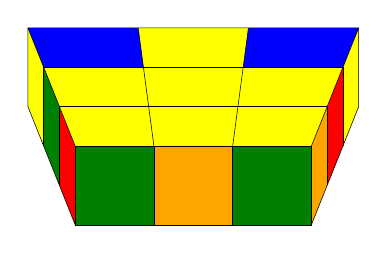
\begin{tikzpicture}
    % --- --- --- Up yellow cross
    \fill[\cU] (1,3) -- ++({-(\asp-1)/2},3*\dep) -- ++(\asp,0) -- (2,3) -- cycle;
    \fill[\cU] (0,3) ++ ({-(\asp-1)/2},\dep) -- ++ ({-(\asp-1)/2},\dep) -- ++(2*\asp+1,0) -- ++({-(\asp-1)/2},-\dep) -- cycle;
    % --- --- --- LBU corner
    \fill[\cU] (0,2) ++({-(\asp-1)/2*3},3*\dep) -- ++(0,1) -- ++({+(\asp-1)/2},-\dep) -- ++(0,-1) -- cycle;
    \fill[\cB] (0,3) ++({-(\asp-1)/2*3},3*\dep) -- ++(\asp,0) -- ++({+(\asp-1)/6},-\dep) -- ++({-(2*\asp+1)/3},0) -- cycle;
    % --- --- --- RBU corner
    \fill[\cU] (3,2) ++({+(\asp-1)/2*3},3*\dep) -- ++(0,1) -- ++({-(\asp-1)/2},-\dep) -- ++(0,-1) -- cycle;
    \fill[\cB] (3,3) ++({+(\asp-1)/2*3},3*\dep) -- ++(-\asp,0) -- ++({-(\asp-1)/6},-\dep) -- ++({+(2*\asp+1)/3},0) -- cycle;
    % --- --- --- FLU corner
    \fill[\cF] (0,2) rectangle (1,3);
    \fill[\cL] (0,2) -- ++({-(\asp-1)/2},\dep) -- ++(0,1) -- ++({+(\asp-1)/2},-\dep) -- cycle;
    \fill[\cU] (0,3) -- ++({-(\asp-1)/2},\dep) -- ++({(\asp+2)/3},0) -- ++({+(\asp-1)/6},-\dep) -- cycle;
    % --- --- --- FRU corner
    \fill[\cF] (2,2) rectangle (3,3);
    \fill[\cR] (3,2) -- ++({+(\asp-1)/2},\dep) -- ++(0,1) -- ++({-(\asp-1)/2},-\dep) -- cycle;
    \fill[\cU] (3,3) -- ++({+(\asp-1)/2},\dep) -- ++({-(\asp+2)/3},0) -- ++({-(\asp-1)/6},-\dep) -- cycle;
    % --- --- --- FU edge
    \fill[\cR] (1,2) rectangle (2,3);
    % --- --- --- LU edge
    \fill[\cF] (0,2) ++({-(\asp-1)/2},\dep) -- ++({-(\asp-1)/2},\dep) -- ++(0,1) -- ++({+(\asp-1)/2},-\dep) -- cycle;
    % --- --- --- RU edge
    \fill[\cL] (3,2) ++({+(\asp-1)/2},\dep) -- ++({+(\asp-1)/2},\dep) -- ++(0,1) -- ++({-(\asp-1)/2},-\dep) -- cycle;
    % === === === Front
    \draw[very thin] (0,2) rectangle (3,3);
    \draw[very thin] (1,2) rectangle (2,3);
    % === === === Up
    \draw[very thin] (0,3) -- ++({-(\asp-1)/2*3},3*\dep) -- ++(3*\asp,0) -- ++({-(\asp-1)/2*3},-3*\dep);
    \draw[very thin] (0,3) ++ ({-(\asp-1)/2*1},1*\dep) -- ++(1*\asp+2,0);
    \draw[very thin] (0,3) ++ ({-(\asp-1)/2*2},2*\dep) -- ++(2*\asp+1,0);
    \draw[very thin] (1,3) -- ({1*\asp-(\asp-1)/2*3},3+3*\dep);
    \draw[very thin] (2,3) -- ({2*\asp-(\asp-1)/2*3},3+3*\dep);
    % === === === Left
    \draw[very thin] (0,2) -- ++({-(\asp-1)/2*3},3*\dep) -- ++(0,1);
    \draw[very thin] (0,2) ++({-(\asp-1)/2*1},1*\dep) -- ++(0,1);
    \draw[very thin] (0,2) ++({-(\asp-1)/2*2},2*\dep) -- ++(0,1);
    % === === === Right
    \draw[very thin] (3,2) -- ++({+(\asp-1)/2*3},3*\dep) -- ++(0,1);
    \draw[very thin] (3,2) ++({+(\asp-1)/2*1},1*\dep) -- ++(0,1);
    \draw[very thin] (3,2) ++({+(\asp-1)/2*2},2*\dep) -- ++(0,1);
\end{tikzpicture}
\end{document}
